\subsection{Reassess Overload Decision}

\subsubsection*{Ausgangslage}

Ein System verwendet Fault Correlation (12), um eine Überlastung abzuwenden. Deshalb wird Deferrable Work (43), Finish Work in Prograss (54) und Shed Load (49) angewandt. Die Überlastung verringert sich aber nicht.

\subsubsection*{Lösungsansatz}

Falls erkannt wird, dass die Überlastung trotz der Versuche diese abzuwenden gleich bleibt oder gar zunimmt, kann es sein, dass die Überlastung nur eine Effekt eines Fehlers ist, der behandelt werden muss. Nimmt die Überlastung zu, muss dies im System festgestellt werden können um weitere respektive andere Massnahmen zu ergreifen.

\subsubsection*{Schlussfolgerung}

Es soll ein Feedback-Loop vorhanden sein, der es ermöglicht, die gefällten Entscheidungen zu korrigieren. Dies ermöglicht es dem System, eine andere Fehlerbehandlung durchzuführen, falls der gewünschte Effekt durch die gewählte Strategie nicht erreicht wird.

\begin{figure}[H]
	\centering
	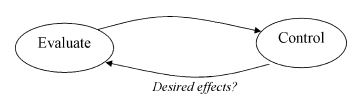
\includegraphics[width=\textwidth]{content/faulttolerance/images/ReassessOverloadDecision.JPG}
	\caption{ReassessOverloadDecision}
\end{figure}


\subsubsection*{Verwandte Patterns}

Anwendung von:
\begin{itemize}
	\item Escalation (9)
\end{itemize}

\begin{itemize}
	\item Someone in Charge (8)
\end{itemize}



